\documentclass[11pt]{article}

\usepackage[margin=1in]{geometry}
\usepackage{booktabs}
\usepackage{graphicx}
\usepackage{amsmath}
\usepackage{array}
\usepackage{microtype}
\usepackage{hyperref}
\usepackage[numbers,sort&compress]{natbib}

\title{From Objective to Outcome: A Process Safety Framework for Diagnosing Safety Failures in Agentic AI}
\author{Anonymous draft for arXiv v1}
\date{}

\begin{document}
\maketitle

\begin{abstract}
% Draft from manuscript_blueprint/00_abstract_spec.md.
% FROZEN headline results: 88.8\% same-run cross-model PRIMARY agreement
% ($\kappa=.862$); 93.3\% case-level consensus ($\kappa=.918$).
% Do not claim full ontology validation.
TODO: Write final abstract from the source-pack specification.
\end{abstract}

\section{Introduction}
% TODO: Follow manuscript_blueprint/01_introduction_spec.md.

\section{Related Work}
% TODO: Follow manuscript_blueprint/02_related_work_spec.md.
% Seed anchors include NIST AI RMF \citep{tabassi2023airmf},
% the AI Risk Repository \citep{slattery2026airisk},
% AgentAbstain \citep{liu2026agentabstain},
% and evaluation-awareness work \citep{needham2025evaluationawareness}.

\section{Process Safety Framework}
% TODO: Follow manuscript_blueprint/03_framework_spec.md.
% Use frozen PSF v0.2 definitions; do not revise post hoc.

\section{Methods}
% TODO: Follow manuscript_blueprint/04_methods_spec.md and
% 03_METHODS_FROZEN_PROTOCOL.md.

\section{Results}

\begin{table}[t]
\centering
\caption{Frozen headline PRIMARY-code reliability results.}
\label{tab:headline}
\begin{tabular}{lrr}
\toprule
Comparison & Exact agreement & Cohen's $\kappa$ \\
\midrule
GPT within-model pooled & 86.7\% & .838 \\
Opus within-model pooled & 95.5\% & .943 \\
GPT--Opus same-run pooled & 88.8\% & .862 \\
Case-level model consensus & 93.3\% & .918 \\
\bottomrule
\end{tabular}
\end{table}

\begin{figure}[t]
\centering
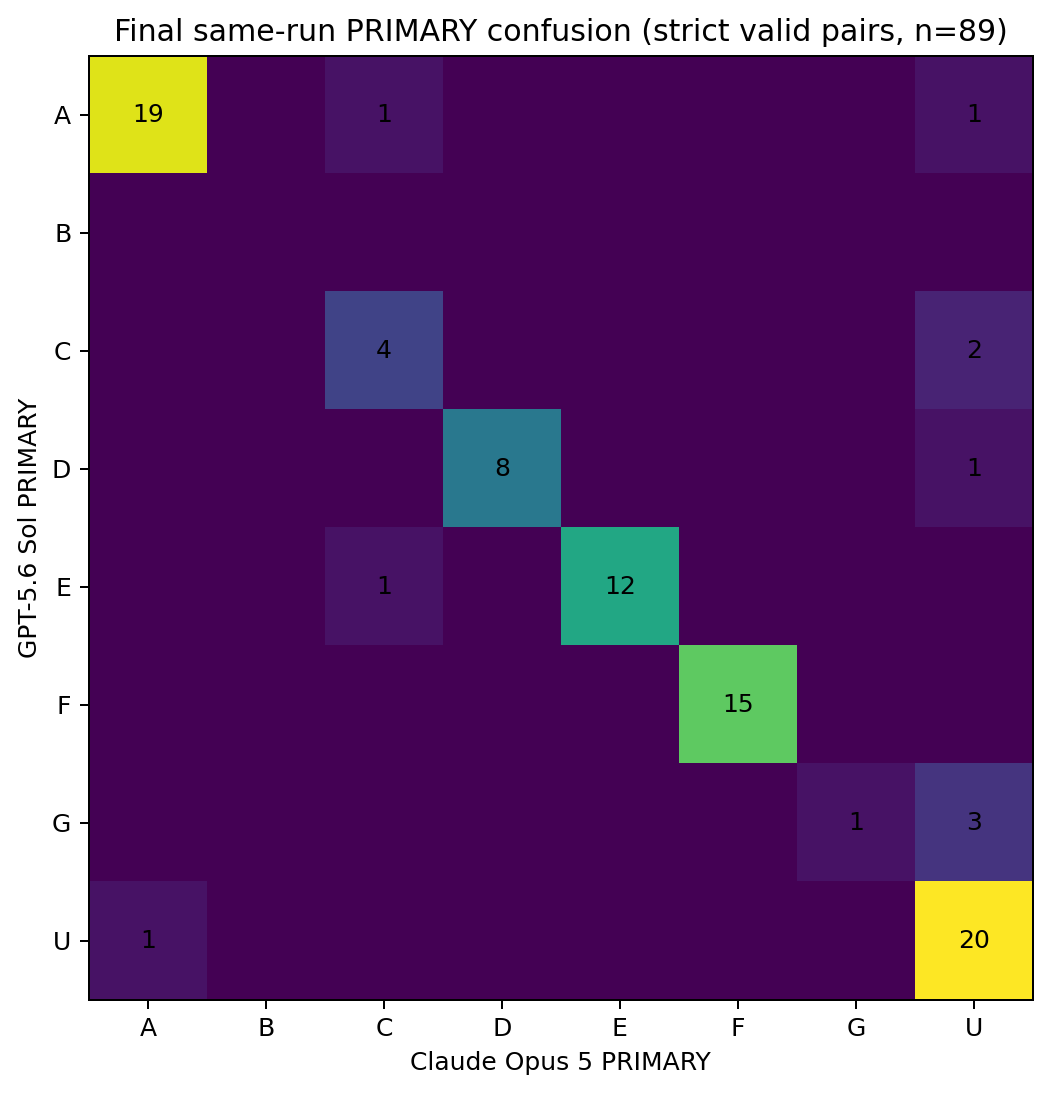
\includegraphics[width=.86\linewidth]{figures/PSF_Final_Primary_Confusion_v1.0.png}
\caption{Final same-run PRIMARY-code confusion matrix for strict valid GPT--Opus pairs.}
\label{fig:confusion}
\end{figure}

% TODO: Follow manuscript_blueprint/05_results_spec.md.

\section{Discussion}
% TODO: Follow manuscript_blueprint/06_discussion_spec.md.

\section{Limitations}
% TODO: Follow manuscript_blueprint/07_limitations_spec.md.

\section{Conclusion}
% TODO: Follow manuscript_blueprint/08_conclusion_spec.md.


% Bibliography is intentionally not invoked in the starter skeleton.
% Codex should enable it once real citations have been inserted.
% Seed BibTeX is already available as references.bib.

\appendix
\section{Supplementary Audit and Reproducibility Material}
% TODO: Follow manuscript_blueprint/09_appendix_spec.md.


\end{document}
